%!TEX root = ../dokumentation.tex

\chapter{Hazelcast (Key-Value)} \label{ch:hazelcast}
\chapterauthor{Nick Schroeder, Maxime Fritzsch, Michelle Mersch}

Exercitation qui duis voluptate do esse aute. Minim deserunt ex minim sunt cupidatat est fugiat in pariatur ullamco. Enim esse voluptate nulla et sunt sint labore non ut eiusmod et. Deserunt laboris ullamco occaecat esse reprehenderit anim. Deserunt aute laboris tempor est occaecat duis in cupidatat.

\section{Introduction} \label{sec:introductionHazelcast}

\section{Fundamentals} \label{sec:fundamentalsHazelcast}
\subsection{History} \label{subsec:historyHazelcast}
Hazelcast is a distributed In-Memory Data Grid platform, developed for Java. It was created by a company of the same name, 
which was founded in 2008 by Talip Ozturk and Fuad Malikov. \cite{DatabaseofDatabases.11032023} The company's headquarters are 
in Palo Alto, California and it also has two European offices in London and Istanbul. \cite{HazelcastContact.03112022} \newline
After its founding in 2008, the company first released an open-source version of Hazelcast in 2009 and has since been updating it 
continously. \cite{DatabaseofDatabases.11032023} Since this first version, Hazelcast has been used by many well known companies, 
among them Intel and IBM, the former of which collaborates with Hazelcast on the optimization of in-memory computing solution, while 
the later has a joint initiative with Hazelcast to create and optimize cloud-native applications. \cite{HazelcastPartners.270122}
\subsection{Capabilities} \label{subsec:capabilitiesHazelcast}
Hazelcast has several features which make it stand out from other solutions to store data, the first of which is how easy it is 
to set Hazelcast up and get it running. This is due to the fact that Hazelcast is self-discovering and self-clustering as Hazelcast's 
Clusters are formed from different nodes which are all functionally the same, operate in a peer-to-peer fashion and are responsible for 
certain data to which they are assigned by the oldest node. \cite{Johns.2015} \newline
Another important feature of Hazelcast is the fact that it persists data completely in memory, which makes Hazelcast very fast and efficient.
While this is one of the often cited advantages of Hazelcast, it also has the disadvantage of the data being lost if nodes are shut down. To counteract this, Hazelcast usually has copies of data on several different node, which makes the failure of a single node less critical as the data doesn't get completely lost and can be immediately saved as a backup 
in another node. This is depicted in \autoref{fig:hazelcast:example_partitioning}, which shows how the overall data is partitioned into three parts, each of which gets saved by two of the tree nodes. Thus, only if more than 
one node fails at exactly the same time data can be lost as the standard count of backup nodes is only 1. This can also be increased though if users want to 
ensure that their data won't get lost, although this requires more node to be operated at the same time. \cite{Johns.2015} \newline

\begin{figure}[H]
    \centering
    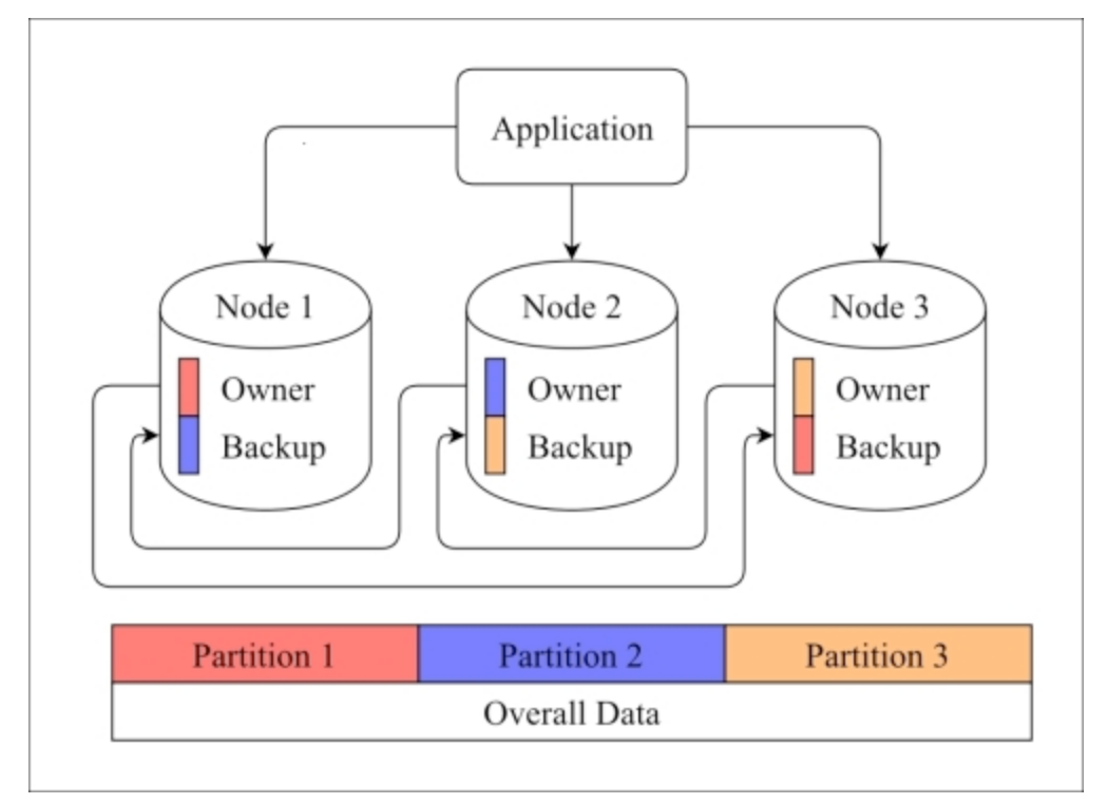
\includegraphics[width=16cm]{images/hazelcast_partitioning.png}
    \caption[Example for partitioning in Hazelcast]{Example for partitioning in Hazelcast, \cite{Johns.2015}}
    \label{fig:hazelcast:example_partitioning}
\end{figure}

Another capability of Hazelcast is its diverse offering of ways to store data, including standard utility collections like lists, sets and queues as well as maps, which enable users to save data as key-value pairs. Additionally to those basic Maps, Hazelcast also offers  
specialized collections like Multi-Maps, which allow for multiple values per key. \cite{Johns.2015}
\subsection{Fields of Application} \label{subsec:fieldsOfApplicationHazelcast}

Hazelcast can be used in numerous different ways, one of which would be to hold data for user sessions, an application that makes sense due to its nature 
of persisting data only in memory and it thus being well suited for working with temporary data. Furthermore, another application of Hazelcast is 
running it together with some data store which persists data long term, leading to an increased capacity. Additionally, Hazelcast in general is well 
suited for applications which require a high performance and elastic scalability as those are both requirements Hazelcast fulfills due to it saving data in memory and 
its automatic clustering. \cite{Johns.2015} \newline


\section{Implementation} \label{sec:implementationHazelcast}
\subsection{Requirements} \label{subsec:requirementsHazelcast}
\subsection{Installation} \label{subsec:installationHazelcast}
\subsection{Python Client} \label{subsec:pythonClientHazelcast}
\subsection{Data Access} \label{subsec:dataAccessHazelcast}

\section{Reflection} \label{sec:reflectionHazelcast}
\subsection{Advantages \& Disadvantages} \label{subsec:advantagesDisadvantagesHazelcast}
\subsection{CAP Theorem} \label{subsec:capTheoremHazelcast}
\subsection{Conclusion} \label{subsec:conclusionHazelcast}

